\chapter{Fussballszenario} \label{kap:Fussballszenario} %TODO: Besseren Kapiteltitel

\section{Szenario Koordination}  %TODO: Hendrik
\sectionauthor{H.O.}

Die Szenario Koordination umfasst sowohl das Verhalten der einzelnen AMiRos, kooperative Elemente zwischen verschiedenen AMiRos als auch die Kommunikation mit dem Host-PC. Der Entwurf dieser drei Themenbereiche sollen im folgenden kurz vorgestellt und begründet werden:\\
Um ein bestimmtes Verhalten zu zeigen, müssen die AMiRos selbst zunächst über einen Satz einzelner Fähigkeiten verfügen. Ein komplexeres Verhalten entsteht dann aus der Kombination der einzelnen Fähigkeiten, indem diese sequenziell oder parallel miteinander kombiniert werden. Denkbar wäre ebenso die Realisierung einer Verhaltenshierarchie, in der sich einzelne Verhaltensweisen beeinflussen und sich gegenseitig unterdrücken oder verstärken können. Ein solcher Ansatz wird näher in \cite{Brooks:1986} beschrieben.\\
Da das Szenario in seiner Komplexität jedoch noch begrenzt ist und kein vollständig generisches Verhalten implementiert werden musste, wurde für die Umsetzung im Projektkontext durch eine einfache State-Machine realisiert. Die Zustände stellen einzelne Verhaltensweisen des Roboters dar und durch bestimmte Nachrichten (Events) kann zwischen ihnen gewechselt werden.\\
Das Verhalten einzelner AMiRos wird erweitert durch kooperative Fähigkeiten und die Möglichkeit der Kommunikation durch einen festgelegten Befehlssatz. Kann beispielsweise ein AMiRo während einer Spielaktion den Ball nicht lokalisieren, kann er eine Nachricht an den anderen AMiRo schicken, woraufhin dieser sich dann ein Stück bewegt, um die Sicht auf den Ball freizugeben.\\
Zusätzlich besteht die Möglichkeit für die AMiRos mit dem Host-PC zu kommunizieren, der an Hand eines Kamerabildes und zusätzlicher Bildverarbeitungslogik das Spielgeschehen verfolgen, interpretieren und steuern kann. Dies erlaubt außerdem eine Benutzerinteraktion um das Spiel zu starten, zu pausieren oder zu unterbrechen. In der derzeitigen Realisierung übermittelt der Host-PC außerdem noch den Status des Spielballs, also ob dieser in Bewegung ist oder ruht. Diese Information wird von den AMiRos verwendet, um eigenständig zu bestimmen, welcher AMiRo gerade am Zug ist.

\vfill

\subsection{Kommunikation per RSB und Spread} %TODO: Hendrik
\sectionauthor{H.O.}
Damit die AMiRos untereinander kommunizieren können, wurde eine Publish-Subscribe Architektur basierend auf der RSB Middleware aufgesetzt und anstatt einer einfachen Socket-Transport Lösung wurde auf das etwas komplexere Spread Toolkit zurückgegriffen (siehe RSB Konfigurationsdatei im Anhang \ref{sec:rsb-config}).\\
Die Publish-Subscribe Architektur bietet den Vorteil der asynchronen Kommunikation, die im Zusammenspiel mit einer State-Machine besonders praktisch ist. Die State-Machine muss nicht auf explizit auf Antworten warten, sondern kann beliebig weiterlaufen und reagiert erst dann, wenn eine Nachricht empfangen wurde. Zudem bietet sie den Vorteil das sehr leicht Software-Komponenten hinzugefügt und an die bestehende Kommunikation angeschlossen werden können (vgl.\cite{Siciliano:2007}).\\
Jeder AMiRo (und auch der Host-PC) hat also eine bestimmte Anzahl an Empfängern (Listener) und Sendern (Publisher) um Nachrichten in bestimmten Geltungsbereichen (Scopes) zu empfangen oder zu senden. Als Nachrichten werden der Einfachheit halber einfache Strings versendet, die dann beim Empfänger geparst werden können. Das Debugging während der Entwicklung wurde so vereinfacht, allerdings hat dieser Ansatz auch Nachteile: Zum einen müssen die Listen an Strings auf Empfänger und Senderseite immer gepflegt werden, damit sie identisch sind und ein zuverlässiges Parsen erlauben. Zum anderen bieten gekapselte Nachrichten mehr Typensicherheit und ggf. auch die Option zusammengehörige Informationen zu kapseln. Im Umfang des Projekt war die Wahl lediglich einfach Strings zu übertragen durchaus ausreichend, die Lösung skaliert aber nicht für größere Projekte.\\
Das Spread Toolkit hilft dabei einen Nachteil der allgemeinen Publish-Subscriber Architektur zu beseitigen: Die Kommunikation beruht nicht auf einem zentralen Endpunkt, der die gesamte Kommunikation steuert, sondern jeder Spread-Daemon überwacht die Verbindungen zu allen anderen Endpunkten und hält diese so aufrecht (vgl.\cite{Siciliano:2007}). So kann auch bei kurzzeitigen Verbindungsabbrüchen sichergestellt werden, dass die Verbindung automatisch wiederhergestellt wird. Auf Programmebene  muss so weniger Overhead für die Sicherstellung der Verbindung implementiert werden und der Code bleibt einfacher und somit besser wartbar.\\
Neben der Plattform-übergreifenden Kommunikation werden RSB und Spread zusätzlich auch für Interprozess-Kommunikation auf den AMiRos und auf dem Host-PC eingesetzt. Wie in Abb. \ref{fig:spread} zu sehen ist, laufen auf beiden AMiRos die drei gleichen Softwarekomponenten. Die State-Machine (FSM) steuert das Verhalten und die Kommunikation. Die locateAndShoot Komponente stellt die Verhaltenseinheiten für das Szenario zur Verfügung und die SearchCharging Komponente erlaubt aus dem Szenario aus die Lokalisation und das Anfahren an die Ladestation. Diese drei Komponenten kommunizieren über den internen Spread, der auf der internen localhost Schnittstelle auf dem Port 4806 läuft (siehe dazu auch Anhang \ref{sec:spread-config}).\\
Die Kommunikation zwischen den AMiRos selbst und dem Host läuft über einen weiteren Spread-Daemon, der mit einer anderen Konfiguration geladen wird, die W-LAN Schnittstelle nutzt und auf Port  4803 hört und sendet (siehe ebenfalls Abschnitt \ref{sec:spread-config}).\\
Die W-LAN Verbindung wurde durch einen eigenen Router realisiert und erlaubt so die feste Adresszuweisung für die drei Endpunkte, damit die Spread-Konfiguration darauf zurückgreifen kann. Die Einzelheiten können der W-LAN Konfiguration im Anhang (\ref{sec:wlan-config}) entnommen werden.
\begin{figure}[H]
	\begin{center}
		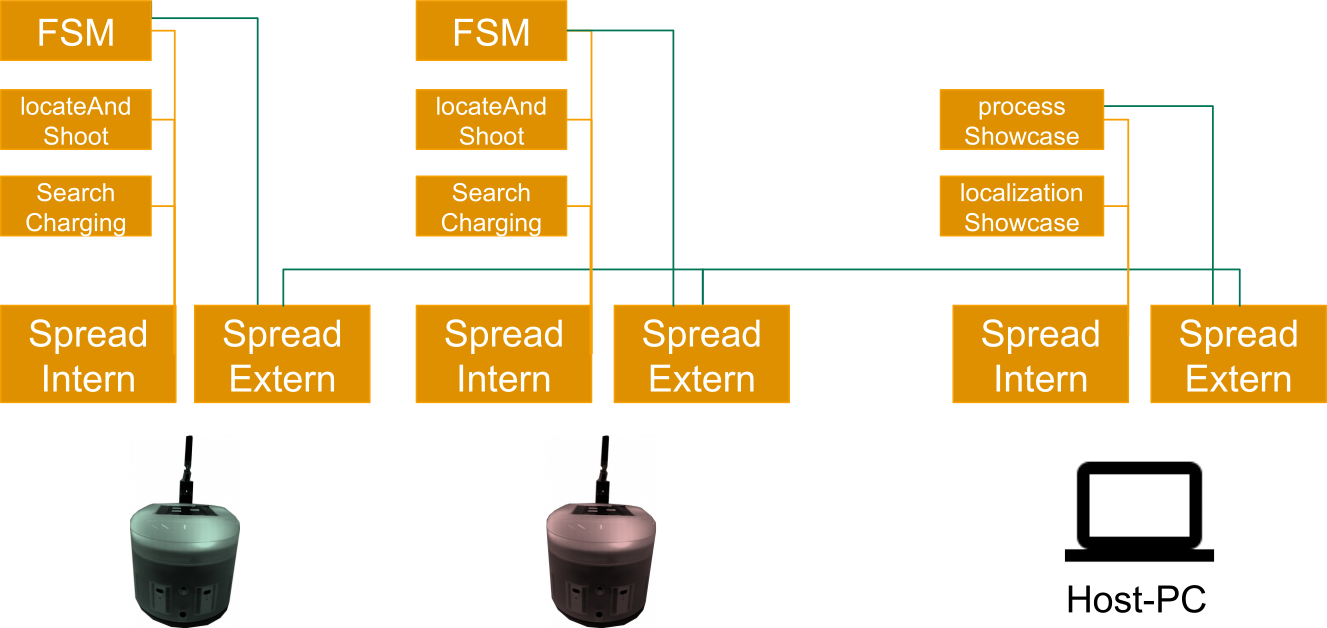
\includegraphics[scale=.65]{spread_communication.png} 	
		\caption{Spread-Kommunikation}
		\label{fig:spread}
	\end{center}
\end{figure}

\subsection{Finite-State-Machine} %TODO: Hendrik
\sectionauthor{H.O.}
Die State-Machine regelt das Verhalten der einzelnen AMiRos. Jedes Verhalten wird in kleinstmögliche Einheiten unterteilt, die dann einzeln angesprochen und überall wiederverwendet werden können. Nach der Initialisierung aller RSB-Komponenten und Variablen wird im Programm die State-Machine gestartet.\\ 
Solange kein Fehler auftritt, bleibt das Programm immer innerhalb der State-Machine und wechselt den aktuellen Zustand nur auf Grund externer Nachrichten, die in Form von RSB Events oder CAN Messages eingehen können. Extern beschreibt also in diesem Zusammenhang sowohl die anderen Programmkomponenten die auf dem AMiRo laufen, als auch RSB Events von einem anderen AMiRo oder dem Host-PC und CAN Nachrichten vom Mikrocontroller.\\
Einzelne Zustände haben auch direkte Anweisungen die den aktuellen Zustand wechseln können, dies soll eine Kapselung der einzelnen Verhaltenseinheiten unterstützen und erlaubt es zukünftige Änderungen oder Erweiterungen leichter durchführen zu können.\\
Die State-Machine selbst ist in Abb. \ref{fig:fsm-amiro} dargestellt. Nach dem Start ist zunächst der \texttt{idle} Zustand aktiv. Dieser wartet lediglich auf Kommandos und stellt sicher, dass sich der AMiRo nicht bewegt, sondern ruhig auf seiner Position abwartet.\\
Um das Spiel zu starten, muss eine Nachricht vom Host-PC an die AMiRos geschickt werden.Der aktuelle Zustand wechselt dann auf \texttt{startScenario}. Hier können Initialisierungen vorgenommen werden, die notwendig sind, damit der Roboter das Spiel antreten kann. In der derzeitigen Implementierung werden beispielsweise die Teamfarben auf den oberen LEDs des AMiRos gesetzt. Eine mögliche Erweiterung des Szenarios wäre beispielsweise, dass die Spieler auch bestimmte Positionen auf dem Spielfeld einnehmen.\\
Ist die Initialisierung abgeschlossen, wechselt die State-Machine in den \texttt{ready} Zustand. In diesem Zustand bleibt die FSM solange, bis der Host-PC das Spiel offiziell startet, doch abbricht oder bis die Ladestrategie das Ladeverhalten anstößt.\\
Wird das Spiel gestartet, ist der \texttt{waitForTurn} State aktiv. Dieser wartet im Normalfall auf die Nachricht eines anderen AMiRos, der seinen Spielzug abgeschlossen hat und somit das Handle an ihn selbst übergibt. Beim Spielstart hingegen versendet der Host-PC einmalig ein Event mit entsprechendem Inhalt und definiert so, welche Roboter beginnen darf. Im normalen Spielverlauf kann es auch passieren, dass der AMiRo dem Gegner die Sicht auf den Ball verdeckt. Signalisiert der Gegner dies durch eine Nachricht, wechselt die State-Machine in den \texttt{moveFromBall} State, sendet dort eine Nachricht an die locateAndShoot Anwendung und wechselt dann wieder zurück in den \texttt{waitForTurn} Zustand. Gleichzeitig wird eine Bestätigungsnachricht an den Gegner verschickt um zu signalisieren, dass die Neupositionierung abgeschlossen ist.\\
Ist der AMiRo selbst an der Reihe, um seinen Spielzug zu machen, beginnt er damit im \texttt{localizeBall} State. Er versucht den Ball zu lokalisieren und wechselt bei erfolglosem Versuch in den \texttt{waitForOtherAmiroMove} Zustand, in dem eine Nachricht an den Gegner geschickt wird, damit dieser sich bewegt. Nach Bestätigung des Gegners, dass dieser seine Position geändert hat, wechselt die FSM wieder in den \texttt{localizeBall} Zustand und versucht erneut die Lokalisierung des Balls. Bei Erfolg wird dann zu \texttt{moveToBall} gewechselt.\\
Die folgenden Zustände verlaufen sequenziell und können daher zusammenfassend beschrieben werden:
\texttt{moveToBall},\texttt{findGoal},\texttt{moveToShootingPosition},\texttt{shootBall}. Jeder dieser Zustände verschickt ein Event an das locateAndShoot Programm, wartet auf erfolgreiche Rückmeldung und wechselt dann in den jeweils nachfolgenden State. Wie auch in den meisten Zuständen zuvor, gibt es zusätzlich noch die Möglichkeit, dass das Spiel abgebrochen wird oder der AMiRo laden muss. Dann wird jeweils in den \texttt{cancelScenario} oder in den \texttt{moveToEdge} State gewechelt.\\
Nachdem der Ball vom Roboter geschossen wurde, muss zunächst auf eine Bestätigung vom Host-PC gewartet werden, bis der Ball sich nicht mehr bewegt. Erst dann soll das Handle an den anderen AMiRo übergeben werden. Der Host-PC sendet allerdings kontinuierlich ein Signal aus, solange sich der Ball bewegt, die State-Machine wartet sicherheitshalber mehrere Durchgänge in denen keine Nachricht vom Host-PC empfangen werden darf, die eine Ballbewegung signalisiert. Erst dann wird das Handle im nachfolgenden State \texttt{giveHandleToOtherAmiro} übergeben. In diesem Zustand ist ein Hand-Shaking Mechanismus eingebaut, um sicherzustellen, dass der Gegner das Handle auch empfangen hat. Ist das der Fall, wird wieder zurück in den \texttt{waitForTurn} Zustand gewechselt.\\
Auch das Ladeverhalten wird aus State-Machine Sicht in mehrere Schritte unterteilt und erlaubt so eine gewisse Flexibilität. Gestartet wird das Ladeverhalten durch den \texttt{moveToEdge} State, der den Roboter aus dem Spielgeschehen heraus lenken soll, bis er die nächste Kante gefunden hat. Ist er dort angekommen wechselt er in den \texttt{waitingAtEdge} Zustand. Je nach dem ob die Ladestation gerade frei ist, kann die FSM dann direkt in den nächsten Zustand übergehen oder muss dort solange warten, bis die Ladestation frei wird. Im \texttt{moveToCharging} Zustand startet der AMiRo eine Kantenverfolgung und versucht dann an Hand bestimmter Merkmale die Ladestation zu lokalisieren, indem er entsprechende RSB Events an die SearchCharging Anwendung sendet. Ist er an der Ladestation angekommen, wechselt die State-Machine in den \texttt{moveIntoStation} State und kommuniziert dann über CAN Nachrichten mit den Mirkocontroller Schnittstellen. Wird so ein erfolgreiches Andocken zurückgemeldet, wird dann (ebenfalls über CAN) das eigentliche Laden gestartet. Der Roboter lädt dann in der Regel vollständig auf, es sei denn er empfängt zwischendurch Notrufsignale von einem anderen AMiRo der einen kritischen Ladezustand erreicht hat. 

\subsection{Ladestrategie} %TODO: Hendrik
\sectionauthor{H.O.}
Während des Szenarios ist es für die Roboter wichtig, ihren eigenen Ladezustand zu überwachen und beim Überschreiten gewisser Grenzwerte ein bestimmtes Verhalten auszulösen. Der aktuelle Ladezustand kann wird bei jedem Durchlauf der FSM über den CAN Bus abgefragt und überprüft. Die genaue Ladestrategie wird in Abb. \ref{fig:charging-strategy} verdeutlicht. Fällt die Ladekapazität unter 10\%  wird zunächst überprüft, ob wie der Ladezustand des anderen AMiRos aktuell ist. Liegt dieser ebenfalls unter 15\% wird das Ladeverhalten gestartet. Fällt die eigene Ladekapazität unter 5\% wird das Ladeverhalten ebenfalls ausgelöst. Wird dann eine weitere Grenze von 2\% unterschritten, wird zusätzlich eine Art Notrufsignal vom AMiRo gesendet, dass einen anderen Roboter der gerade die Ladestation blockiert, aber schon ein bestimmtes Ladelevel erreicht hat dazu anhält seinen Ladevorgang abzubrechen und die Ladestation frei zu machen.

\begin{figure}[H]
	\begin{center}
		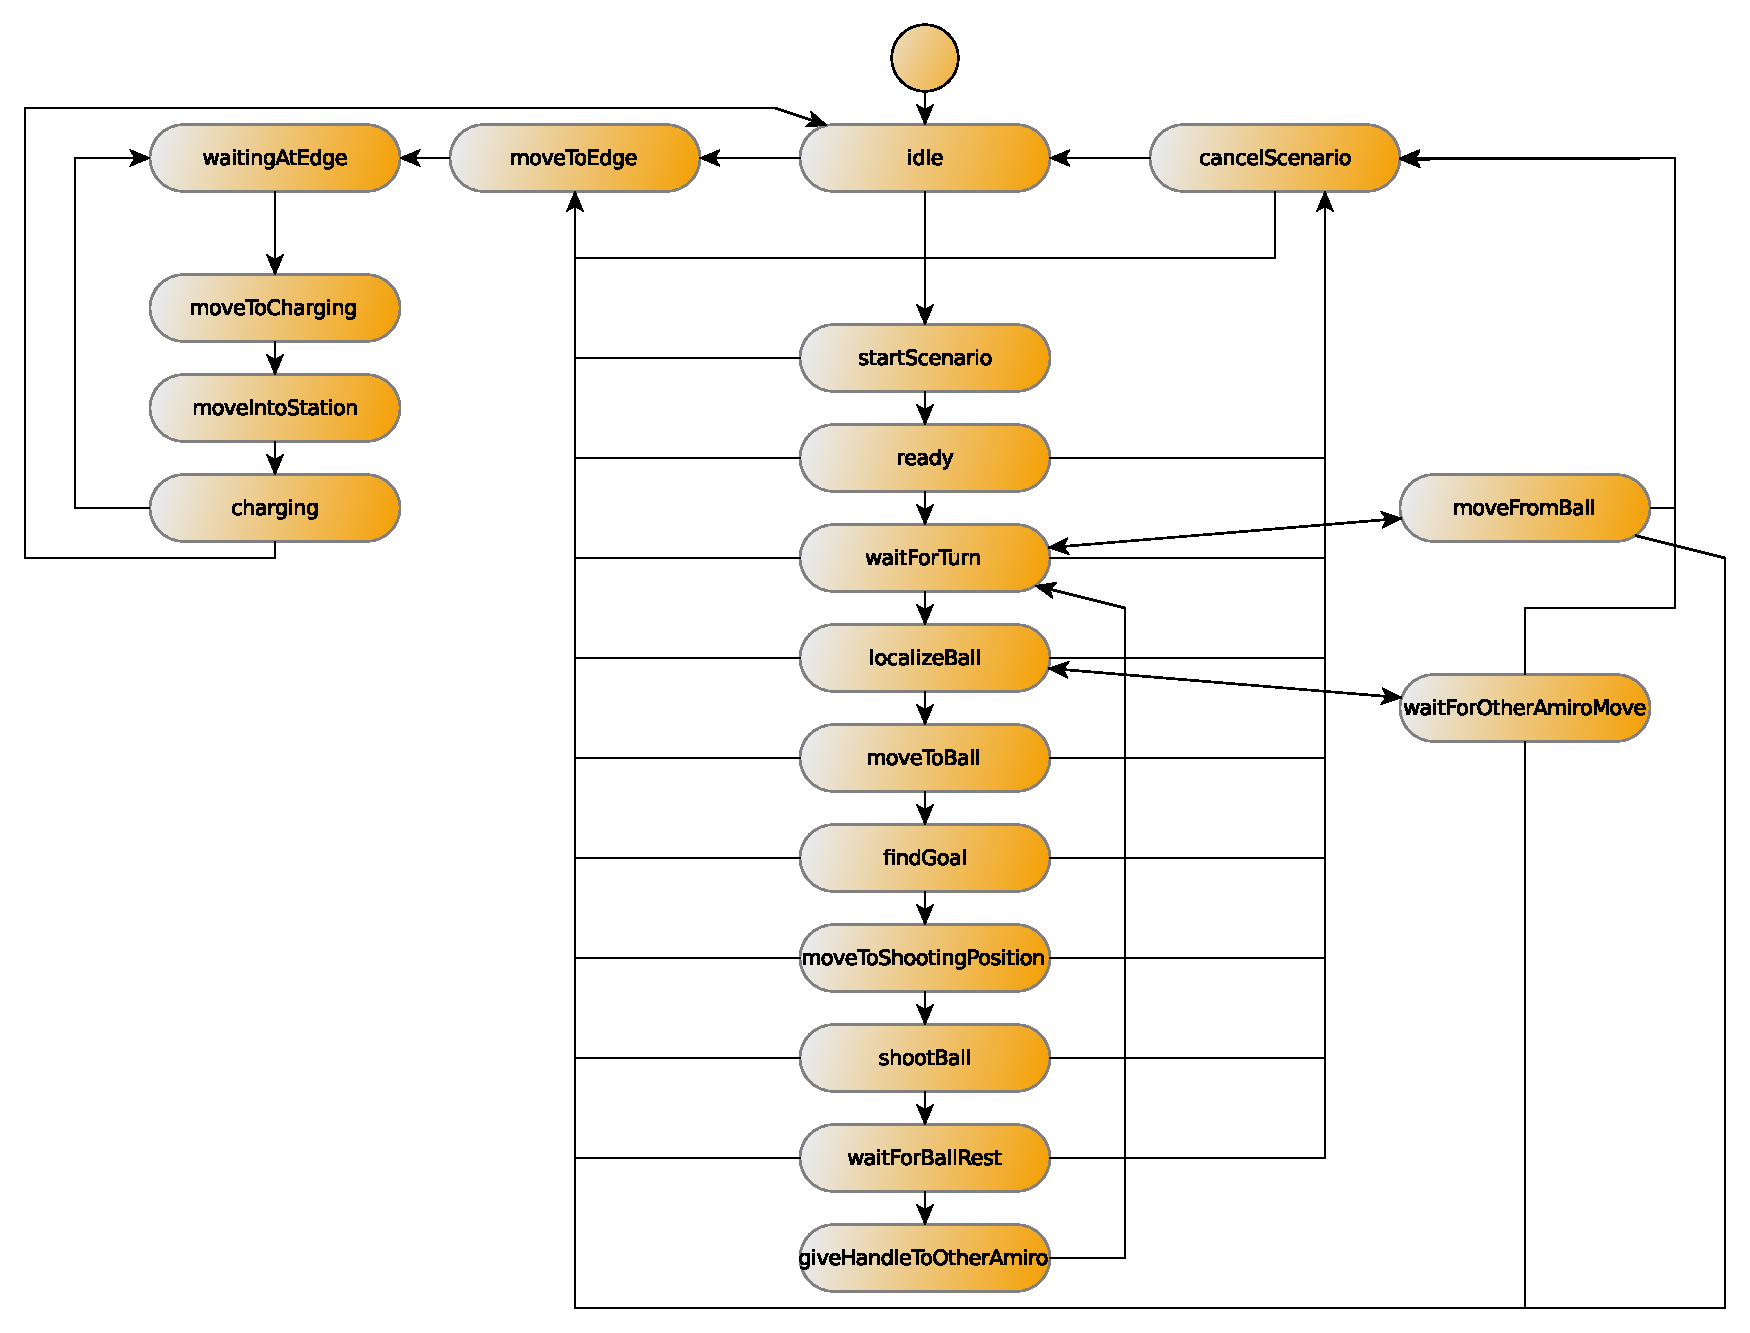
\includegraphics[scale=.55]{Final_FSM_AMiRo.pdf} 	
		\caption{Finite-State-Machine}
		\label{fig:fsm-amiro}
	\end{center}
\end{figure}
\begin{figure}[H]
	\begin{center}
		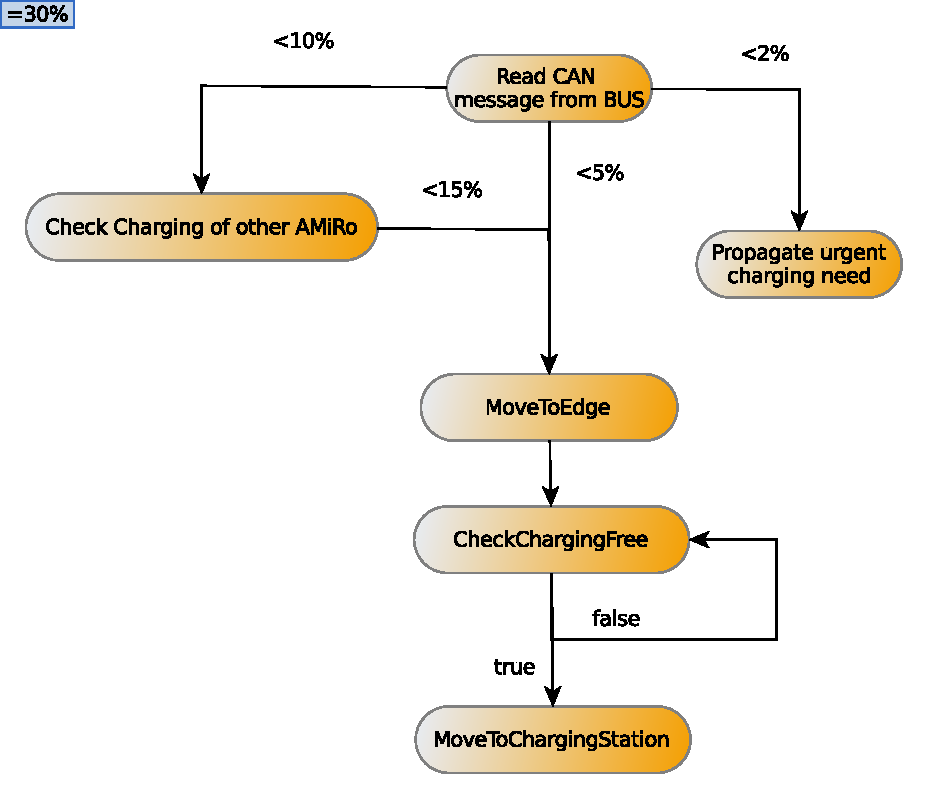
\includegraphics[scale=.50]{Charging_Strategy.pdf} 	
		\caption{Ladestrategie}
		\label{fig:charging-strategy}
	\end{center}
\end{figure}

\section{Realisierung der einzelnen Spielelemente} %TODO: Besseren Sectiontitel

\subsection{Lokalisation des Balls} %TODO: Julian E.
\sectionauthor{J.E.}

\subsection{Anfahren des Balls} %TODO: Julian E.
\sectionauthor{J.E.}

\subsection{Lokalisation des gegnerischen Tores} %TODO: Timo M.
\sectionauthor{T.M.}
- Rotation um eigene Achse zur Lokalisation des Tores
- Lokalisation Anhand von Blobb-Detektion 
- Wenn ein einzelner Pfosten im Bild vorhanden ist - bereits gedrehten Winkel + zusätlichen Winkel vom Mittelpunkt des Bildes zum Pfosten speichern
- Wenn beide Pfosten im Bild vorhanden sind - bereits gedrehten Winkel + zusätlichen Winkel vom Mittelpunkt des Bildes zum Tormittelpunkt speichern und Rotation beenden
- Drehung zum Ball durchführen, um diesen wieder vor sich zu haben

\subsection{Schussposition anfahren} %TODO: Timo M.
\sectionauthor{T.M.}
- Je nach Winkel zum Tor entscheiden, ob der Ball links- oder rechtsseitig umfahren werden soll
- 90$^\circ$ Drehung zu der gegebenen Seite 
- Umfahren des Balles bis vorher berechneter Winkel zum Tor erreicht ist
	- Bei einem Hindernis wird das Umfahren des Balles gestoppt
- 90$^\circ$ Drehung zum Ball
- Überprüfung, ob sowohl Ball als auch das Tor im Bild zu sehen ist 
	- Ist dies der Fall -> feinjustierung der Schussposition 

\subsection{Schießen} %TODO: Timo M.
\sectionauthor{T.M.}
- Überprüfen der seitlichen vorderen Abstandssensoren ob eine Wand detektiert wird
	- Sollte eine Wand auf einer Seite detektiert werden -> Angedrehter Schuss mit Drehung des AMiRos weg von der Wand
- Schießen des Balles durch kurzes Ansteuern beider Motoren 

\subsection{Beiseite Fahren} %TODO: Julian E. (Besseren Titel suchen^^)
\sectionauthor{J.E.}

\subsection{Torjubel} %TODO: Andreas G.
\sectionauthor{A.G.}

\section{Spieltracking} %TODO: Julian D.
\sectionauthor{J.D.}

\subsection{Spielfeldbestimmung mit dem AR Toolkit} %TODO: Julian D.
\sectionauthor{J.D.}

\subsection{Extraktion wichtiger Spielelemente mit Bildverarbeitungsmethoden} %TODO: Julian D.
\sectionauthor{J.D.}

\subsection{Benutzerinteraktion mit AR Markern} %TODO: Julian D.
\sectionauthor{J.D.}

\subsection{Spielkoordination} %TODO: Julian D.
\sectionauthor{J.D.}

\subsection{Grafische Darstellung der Spielstatus} %TODO: Julian D.
\sectionauthor{J.D.}